\synctex=1

% ############ Global ############

\documentclass[%
    fontsize=11pt,
	paper=A4,
	parskip=half,
	DIV=calc,
	headinclude=true,
	footinclude=true,
	footheight=0cm,						% remove space under footer
	appendixprefix=true,
	bibliography=totoc,					% bibintoc
	open=right,
	oneside,
    german
]{scrbook}
\usepackage[utf8]{inputenc}				% German Umlaut- and language support
\usepackage[german]{babel}
\usepackage[T1]{fontenc}
\usepackage{csquotes}					% Use quotes of the correct language
\newcommand{\myAuthor}{InsertShortAuthorHere}
\author{
	Lastname, Surname\\
	\texttt{this-is-my-email@stud.hs-offenburg.de}
	\and
	Lastname, Surname\\
	\texttt{this-is-my-email@stud.hs-offenburg.de}
	\ \\\\
}
\newcommand{\myTitle}{InsertTitleHere}
\title{\myTitle}
\subtitle{InsertSubtitleHere}
\newcommand{\myCourse}{UNITS X}
\newcommand{\myProject}{InsertProjecthere}
\newcommand{\myUniversity}{Hochschule Offenburg}
\newcommand{\myInstitutehead}{University of Applied Sciences}
\newcommand{\mySupervisor}{InsertProfHere}
\newcommand{\myKeywords}{Keyword1, Keyword2}
				% Basic information

% ############ Seite/Header + Footer ############

\usepackage[automark,headsepline,footsepline]{scrlayer-scrpage}			% Header + Footer
\pagestyle{scrheadings}								% for customization for header and footer
\renewcommand{\chapterpagestyle}{scrheadings}					% include header and footer on chapter pages
\clearscrheadfoot								% avoid double page numbers
\automark{chapter}
\ihead{\headmark}
\ifoot{\vspace{-0.25cm}\myTitle, \myAuthor}
\ofoot{ \vspace{-0.25cm} \thepage}

\usepackage[hang]{footmisc} 							% Footnotes space between number and content
\usepackage{calc}								% Header Footer calculation
%Normal
\usepackage[left=1.7cm,right=1.7cm,top=2.7cm,bottom=2.7cm,footskip=0.5cm]{geometry}
%BCOR 8mm
%\usepackage[left=2.1cm,right=1.3cm,top=2.7cm,bottom=2.7cm,footskip=0.5cm]{geometry}

\renewcommand{\chapterheadstartvskip}{}						% remove vertical space before chapter

\usepackage{chngcntr}								% dont't reset footnote enumeration per  chapter
\counterwithout{footnote}{chapter}

% ############ Farben ############

\usepackage[table, usenames, dvipsnames]{xcolor}

\setkomafont{footsepline}{\color{HSColor}} 	 				% change colors of seperation lines
\setkomafont{headsepline}{\color{HSColor}}
\definecolor{DispositionColor}{RGB}{0,0,0}							
\definecolor{light-gray}{gray}{0.95}
\definecolor{dark-green}{rgb}{0,0.6,0}
\definecolor{NiceRed}{HTML}{EF3723}
\definecolor{NiceBlue}{HTML}{4586DF}
\definecolor{NiceGreen}{HTML}{00BD60}
\definecolor{NiceYellow}{HTML}{FCEC0F}


%\definecolor{LinkColor}{HTML}{ba0000}	% toc
\definecolor{UrlColor}{HTML}{155196}	% url
\definecolor{CiteColor}{HTML}{6200d9}	% cite (footnote references to first source)
\definecolor{HSColor}{HTML}{003F61}	% HS Color (toc, footnoteline)

% ############ Schriftart ############

\usepackage{lmodern}								% Latin modern font

\renewcommand{\headfont}{\normalfont\sffamily\color{DispositionColor}}
\renewcommand{\pnumfont}{\normalfont\sffamily\color{DispositionColor}}
\addtokomafont{disposition}{\color{DispositionColor}}
\addtokomafont{caption}{\color{DispositionColor}\footnotesize}
\addtokomafont{captionlabel}{\color{DispositionColor}}

\usepackage[%									% Increase font quality
protrusion=true, %
factor=900       %
]{microtype}

% ############ Bilder ############

\usepackage[pdftex]{graphicx}
\addtokomafont{caption}{\small} 						% small captions
\usepackage[font=small, labelfont=bf]{caption} 					%textwidth and format options break multiple images in a row
\usepackage{subfig}								% caption und subfig break \footcite in captions. Workaround: \footnotemark in caption and \footcitetext{} below
\usepackage{float}								% force the placement of graphics in text
\usepackage{wrapfig}

% ############ Source Code ############

\usepackage{listings}

% Syntax Highlighting JSON
\lstdefinelanguage{genesis}{
	morestring=[s]{"}{"},
	stringstyle=\color{red},
	comment=[l]{:},
	commentstyle=\color{black},
	literate=
	*{\{}{{{\color{black}{\{}}}}{1}
	{\}}{{{\color{black}{\}}}}}{1}
	{,}{{{\color{black}{,}}}}{1},
	%{,}{{{\color{black}{,}}}}{1}
	%{\{}{{{\color{black}{\{}}}}{1}
	%{\}}{{{\color{black}{\}}}}}{1},
}

\lstset{%
	basicstyle=\footnotesize\ttfamily,	
	keywordstyle=\color{blue},	 %default colors if predefined language is matched
	commentstyle=\color{dark-green},
	stringstyle=\color{red},
	extendedchars=true,
	captionpos=b,
	backgroundcolor=\color{light-gray},
	breakatwhitespace=false,
	breaklines=true,
	showspaces=false,                % dont show spaces as underscore
	showtabs=false,                  % dont show tabs as underscore
	showstringspaces=false,		 % dont show stringspaces as underscore
	tabsize=2,
	escapeinside={\%*}{*)},          % if you want to add LaTeX within your code
	frame=lines,                     % adds a frame around the code
	keepspaces=true,                 % keep code ident (possibly needs columns=flexible)
	numbers=left,                    % line numbers (none, left, right)
	numbersep=8pt,                   % how far the line-numbers are from the code
	numberstyle=\tiny\color{gray},   % line-number style
	rulecolor=\color{black},         % frame always black
	stepnumber=1,                    % number every line
	title=\lstname,                  % use filename as title
	numberbychapter=false,
	literate=%			 % escape äöüß
	{Ö}{{\"O}}1
	{Ä}{{\"A}}1
	{Ü}{{\"U}}1
	{ß}{{\ss}}1
	{ü}{{\"u}}1
	{ä}{{\"a}}1
	{ö}{{\"o}}1
}

% Create framed, shaded, or differently highlighted regions that can 
% break across pages.  The environments defined are 
% \begin{itemize}
%   \item framed: ordinary frame box (\verb+\fbox+) with edge at margin
%   \item shaded: shaded background (\verb+\colorbox+) bleeding into margin
%   \item snugshade: similar
%   \item leftbar: thick vertical line in left margin
% \end{itemize}
\usepackage{framed}

% ############ Tabellen ############

\usepackage{booktabs}				% Table rules (\toprule \midrule \bottomrule)
\usepackage{tabularx}				% Table width etc
\usepackage{rotating}				% rotate stuff
\renewcommand{\arraystretch}{1.5}		% more vertical space in tabular
\usepackage{makecell} 				% linebreak in cells
\usepackage{multirow}				% merge vertical cells

% ############ Biblatex ############

\usepackage[
backend=biber,
style=verbose,
maxbibnames=99,
]{biblatex}
\addbibresource{sources.bib}

% ############ Plots / Diagramme ############

\usepackage{pgfplots}
\pgfplotsset{
	compat=1.12,
}
\usepackage{tikz}
\usetikzlibrary{shapes,arrows}

% ############ Mathe ############

\usepackage{mathtools}
\usepackage{amssymb}

% ############ Verschiedenes ############

\usepackage[printonlyused]{acronym}		% abbreviations
\usepackage{eurosym} 				% Required to use \euro for the euro symbol.
\usepackage{pifont}  				% Sonderzeichen für Titelseite \ding{}
\usepackage[normalem]{ulem}			% Linien unter Absätzen machbar
\usepackage{eso-pic} 				% place absolute and relative
\usepackage{enumitem}				% enumerations 1., 1.1, 1.1.1 etc.

% ############ PDF ############

% prevent club & widow penalty
\clubpenalty10000
\widowpenalty10000
\displaywidowpenalty10000
\pdfcompresslevel=9 		% 0-10
\usepackage[%
pdftitle={\myTitle},
pdfauthor = {\myAuthor},
pdfsubject = {\myTitle},
pdfkeywords={\myKeywords},
colorlinks={true},				% removes color frames and colors text
linkcolor = HSColor,
urlcolor = UrlColor,
citecolor = CiteColor,
anchorcolor = blue,
pdfcreator={pdfTex},
bookmarks=True, 
bookmarksopen=false,				% Bookmarkcolumn is opened on pdf reader start
pdfpagemode=UseOutlines,			% None, UseOutlines, UseThumbs, FullScreen
plainpages=false 				% correct, if pdflatex complains: ``destination with same identifier already exists''
% pdfpagelabels,
%hidelinks,					% removes color and porder
%breaklinks=true,
]{hyperref}


\begin{document}
{
	\centering
	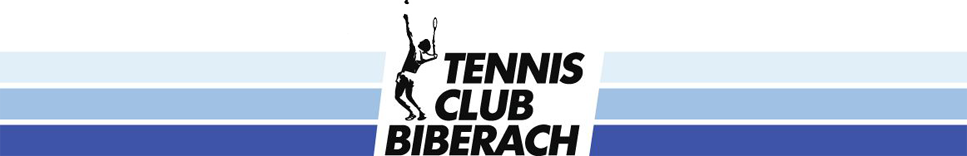
\includegraphics[width=\textwidth]{logo.png}
	\ \\\ \\
}
\begin{Form}
	{
		\huge
		\centering
		\textbf{Beitrittserklärung}\\\ \\
	}
	\noindent
	\begin{tabularx}{\linewidth}{p{9cm} p{9cm}}
		\TextField[name=nachname, width=7cm, bordercolor={black}, borderstyle=U, backgroundcolor=lightergray]{Nachname:\hfill} &
		\TextField[name=vorname, width=7.7cm, bordercolor={black}, borderstyle=U, backgroundcolor=lightergray]{Vorname:\hfill}\\\\
		\TextField[name=strasse, width=7cm, bordercolor={black}, borderstyle=U, backgroundcolor=lightergray]{Straße:\hfill} &
		\TextField[name=plzort, width=7.7cm, bordercolor={black}, borderstyle=U, backgroundcolor=lightergray]{PLZ, Ort:\hfill}\\\\
	\end{tabularx}
	\begin{tabularx}{\linewidth}{p{5cm} p{5.5cm} p{7.5cm}}
		\TextField[name=geb, width=3cm, bordercolor={black}, borderstyle=U, backgroundcolor=lightergray]{Geb.am:\hfill} &
		\TextField[name=tel, width=4cm, bordercolor={black}, borderstyle=U, backgroundcolor=lightergray]{Telefon:\hfill} &
		\TextField[name=mail, width=6cm, bordercolor={black}, borderstyle=U, backgroundcolor=lightergray]{E-Mail:\hfill}\\\\
	\end{tabularx}\\\\
	Ich erkläre hiermit meinen Beitritt zum \textbf{Tennisclub Biberach e.V.} als Mitglied und erkenne die Vereinssatzung an.	Die Mitgliedschaft wird gewünscht als (eines ankreuzen):\\\\
	% TODO \Use ChoiceMenu when hyperref bug is fixed (https://github.com/ho-tex/hyperref/issues/3)
	% set boxes on the left (https://tex.stackexchange.com/questions/446934/latex-forms-place-label-on-the-right-side-of-checkbox)
	\def\LayoutCheckField#1#2{% label, field
		#2 #1%
	}
	\begin{tabularx}{\linewidth}{p{5cm} p{5cm} p{8cm}}
		\CheckBox[name=kinder, bordercolor={black}]{Kinder (bis 13 J.)} &
		\CheckBox[name=jugend, bordercolor={black}]{Jugendliche (14 J. - 17 J.)} &
		\CheckBox[name=azubi, bordercolor={black}]{Azubis, Schüler, Studenten (ab 18 J.)}\\\\
		\CheckBox[name=einzel, bordercolor={black}]{Einzelmitglieder (ab 18 J.)} &
		\CheckBox[name=zweit, bordercolor={black}]{Zweitmitgliedschaft} &
		\CheckBox[name=familie, bordercolor={black}]{Familienmitgliedschaft (inkl. Kinder bis 17 J.)}\\\\
		\CheckBox[name=passiv, bordercolor={black}]{Passiv} &
		\multicolumn{2}{p{13cm}}{\CheckBox[name=schnupper, bordercolor={black}]{Schnuppermitgliedschaft (für laufendes Kalenderjahr, incl. 3 Trainerstunden)}} \\
	\end{tabularx}
	\ \\\\
	\begin{tabularx}{\linewidth}{p{9cm} p{9cm}}
		\TextField[name=ortdatuma, width=7cm, bordercolor={black}, borderstyle=U, backgroundcolor=lightergray]{Ort, Datum:\hfill} &
		Unterschrift: \xrfill[-5pt]{0.5pt}\\\\
		\multicolumn{2}{p{18.4cm}}{Unterschrift gesetzlicher Vertreter (bei Jugendlichen unter 18 Jahren): \xrfill[-5pt]{0.5pt}}
	\end{tabularx}
	\ \\\\{\centering \rule{18.6cm}{2pt}\vspace{0.3cm}}\\
	\textbf{Ermächtigung zum Einzug von Forderungen mittels SEPA-Lastschriftsmandat}\\
	Ich ermächtige den TC Biberach e.V. (Gläubiger ID DE17ZZZ00000301236), Zahlungen von meinem Konto mittels Lastschrift einzuziehen. Zugleich weise ich mein Kreditinstitut an, die von TC Biberach e.V. auf mein Konto gezogenen Lastschriften einzulösen.\\
	Hinweis: Ich kann innerhalb von acht Wochen, beginnend mit dem Belastungsdatum, die Erstattung des belasteten Betrages verlangen. Es gelten dabei die mit meinem Kreditinstitut vereinbarten Bedingungen.\\\\
	\begin{tabularx}{\linewidth}{p{9cm} p{9cm}}
		\TextField[name=kontoinhaber, width=6cm, bordercolor={black}, borderstyle=U, backgroundcolor=lightergray]{Kontoinhaber:\hfill} &
		\TextField[name=bank, width=7.5cm, bordercolor={black}, borderstyle=U, backgroundcolor=lightergray]{Bank:\hfill}\\\\
		\TextField[name=iban, width=7cm, bordercolor={black}, borderstyle=U, backgroundcolor=lightergray]{IBAN:\hfill} &
		\TextField[name=bic, width=7.5cm, bordercolor={black}, borderstyle=U, backgroundcolor=lightergray]{BIC:\hfill} \\\\\\
		\TextField[name=ortdatumb, width=7cm, bordercolor={black}, borderstyle=U, backgroundcolor=lightergray]{Ort, Datum:\hfill} &
		Unterschrift: \xrfill[-5pt]{0.5pt}\\\\
	\end{tabularx}
	\ \\{\centering \rule{18.6cm}{2pt}\vspace{0.3cm}}\\
	\begin{tabularx}{\linewidth}{p{9cm} p{9cm}}
		\multicolumn{2}{p{18.6cm}}{\CheckBox[name=schluessel, bordercolor={black}]{Schlüssel für Platzanlage erhalten}}\\\\
		\TextField[name=ortdatumc, width=7cm, bordercolor={black}, borderstyle=U, backgroundcolor=lightergray]{Ort, Datum:\hfill} &
		Unterschrift: \xrfill[-5pt]{0.5pt}\\\\
	\end{tabularx}
	\begin{center}
		\footnotesize
		Tennisclub Biberach e.V. - 77781 Biberach / Baden\\
		\url{www.tcbiberach.de} $\bullet$ \href{mailto:info@tcbiberach.de}{info@tcbiberach.de}\\\vspace{0.1cm}
		\begin{tabular}{lll}
			Sparkasse Haslach-Zell &
			IBAN: DE17 6645 1548 0027 0200 07 &
			BIC: SOLADES1HAL\\
			Volksbank Lahr eG &
			IBAN: DE85 6829 0000 0045 0293 01 &
			BIC: GENODE61LAH\\
		\end{tabular}
	\end{center}
\end{Form}
\newpage
{
	\centering
	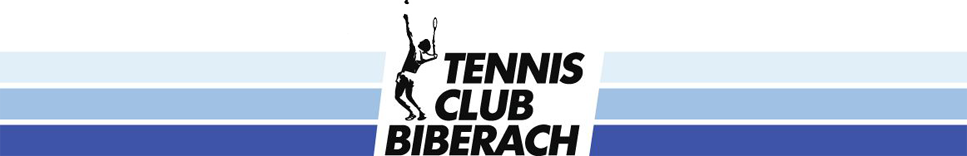
\includegraphics[width=\textwidth]{logo.png}
	\ \\\ \\
}
\begin{Form}
	{
		\huge
		\centering
		\textbf{Datenschutzerklärung}\\\ \\
	}
	\noindent
	\textbf{\Large Allgemeine Vereinbarung}\\
	Die in der Beitrittserklärung angegebenen personenbezogenen Daten, insbesondere Name, Anschrift, Geburtsdatum, Telefonnummer, E-Mail, Bankdaten, die zum Zwecke der Durchführung des entstehenden Mitgliedsverhältnisses notwendig und erforderlich sind, werden auf Grundlage gesetzlicher Berechtigungen erhoben. Diese Informationen werden in dem vereinseigenen EDV-System gespeichert. Jedem Vereinsmitglied wird dabei eine Mitgliedsnummer zugeordnet. Die personenbezogenen Daten werden durch geeignete technische und organisatorische Maßnahmen vor der Kenntnisnahme Dritter geschützt. Vorstandsmitglieder des Vereins sind im Rahmen geltender Beschlüsse des Vorstandes befugt personenbezogene Daten des Mitglieds ausschließlich und alleine für Vereinszwecke zu verarbeiten. Das Mitglied stimmt dieser Art und Weise der Verarbeitung durch seine Mitgliedschaft im Verein zu.\\\\
	\noindent
	\textbf{\Large Pressearbeit}\\
	Der Verein kann über Print- und Telemedien sowie soziale Medien und auf seiner Homepage \url{www.tcbiberach.de} regelmäßig über Turnierergebnisse und besondere Ereignisse (z.B. Ehrungen) informieren.	Dabei können personenbezogene Daten des Mitglieds wie Name, Geburtsdatum, Spielergebnisse, Beitrittsdatum sowie Fotos, die im Rahmen von Aktivitäten des Tennisclub Biberach e.V entstanden sind, veröffentlicht werden. Das einzelne Mitglied kann jederzeit gegenüber dem Vorstand einer solchen Veröffentlichung widersprechen. Im Falle des Widerspruchs unterbleiben in Bezug auf das widersprechende Mitglied weitere Veröffentlichungen. Personenbezogene Daten des widersprechenden Mitglieds werden von der Homepage des Vereins entfernt.\\\\
	\noindent
	\textbf{\Large Austritt aus dem Verein}\\
	Beim Austritt werden die personenbezogenen Daten des Mitglieds archiviert. Personenbezogene Daten des austretenden Mitglieds, die die Kassenverwaltung betreffen, werden gemäß der steuergesetzlichen Bestimmungen bis zu zehn Jahre ab der schriftlichen Bestätigung des Austritts im vereinseigenen EDV-System gespeichert.\\\\
	\noindent
	\textbf{\Large Betroffenenrechte}\\
	Sie sind jederzeit dazu berechtigt die folgenden Rechte ausüben:
	\begin{itemize}
		\setlength\itemsep{0em} % fix spacing between items
		\item Auskunft über Ihre bei uns gespeicherten Daten und deren Verarbeitung (Art. 15 DSGVO)
		\item Berichtigung unrichtiger personenbezogener Daten (Art. 16 DSGVO)
		\item Löschung Ihrer bei uns gespeicherten Daten (Art. 17 DSGVO)
		\item Einschränkung der Datenverarbeitung, sofern wir Ihre Daten aufgrund gesetzlicher Pflichten noch nicht löschen dürfen (Art. 18 DSGVO)
		\item Datenübertragbarkeit, sofern Sie in die Datenverarbeitung eingewilligt haben oder einen Vertrag mit uns abgeschlossen haben (Art. 20 DSGVO)
		\item Widerspruch gegen die Verarbeitung Ihrer Daten bei uns (Art. 21 DSGVO)
	\end{itemize}
	\ \\\\
	\begin{tabularx}{\linewidth}{p{9cm} p{9cm}}
		\TextField[name=ortdatumd, width=7cm, bordercolor={black}, borderstyle=U, backgroundcolor=lightergray]{Ort, Datum:\hfill} &
		Unterschrift: \xrfill[-5pt]{0.5pt}\\\\
		\multicolumn{2}{p{18.4cm}}{Unterschrift gesetzlicher Vertreter (bei Jugendlichen unter 18 Jahren): \xrfill[-5pt]{0.5pt}}
	\end{tabularx}
\end{Form}
\end{document}